\documentclass[a4paper,12pt]{article}
\usepackage[utf8]{inputenc}
\usepackage{graphicx}
\usepackage{amsmath}
\usepackage{amssymb}
\usepackage{pdfpages}
\usepackage[T1]{fontenc}
\usepackage{hyperref}
\usepackage{geometry}
\geometry{a4paper, margin=1in}

\usepackage{graphicx}
\usepackage{booktabs}
\usepackage{float}
\usepackage{listings}
\usepackage[x11names]{xcolor}

\lstdefinestyle{mystyle}{
    backgroundcolor=\color{white},   % 背景颜色
    commentstyle=\color{green},           % 注释颜色
    keywordstyle=\color{blue},            % 关键字颜色
    numberstyle=\tiny\color{gray},        % 行号样式
    stringstyle=\color{purple},              % 字符串颜色
    basicstyle=\ttfamily\footnotesize,    % 基本字体
    breaklines=true,                      % 自动换行
    frame=single,                         % 代码框架
    numbers=left,                         % 显示行号
    captionpos=b,                         % 标题位置
    showstringspaces=false,               % 不显示字符串中的空格
    tabsize=4,                              % 设置制表符宽度
    breaklines = true
}

\lstset{style=mystyle}  





\title{LR(1) Grammar Parser}\date{}
\begin{document}
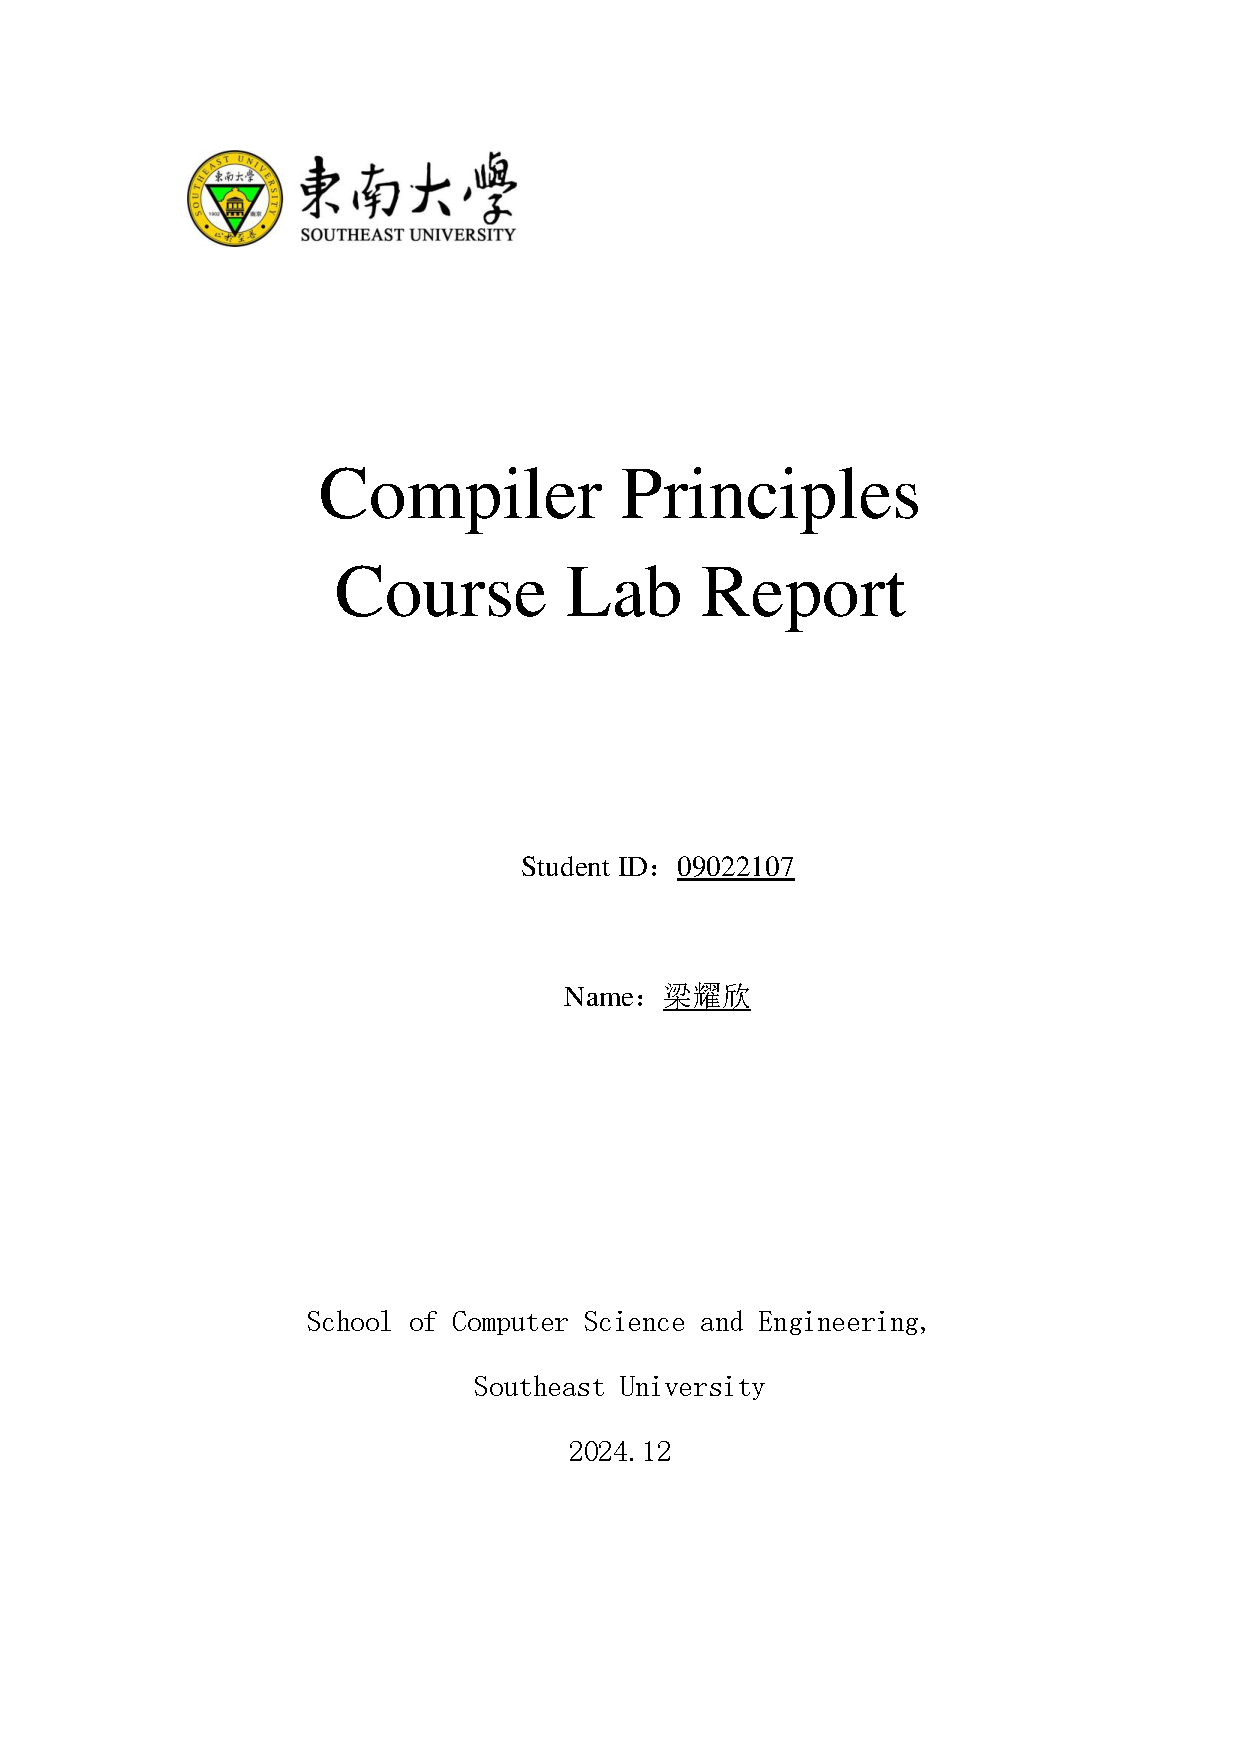
\includepdf[pages=1]{coverage.pdf} 
% 插入目录
\tableofcontents
\newpage
\maketitle

\section{Motivation/Aim}
The aim of this project is to deepen the understanding of the syntax analysis process and implement a syntax analyzer for LR(1) grammars.

\section{Content Description}
\subsection{Non-Programming Implementation}
\begin{enumerate}
    \item \textbf{Define Context-Free Grammar}
    \item \textbf{Draw DFA}: For each state in the DFA, the closure of LR(1) items is constructed, and a tree is built to achieve this. (A photo of the DFA and a related table are provided.)
    \item \textbf{Construct Action and Goto Tables}: Based on the DFA, the Action table and Goto table are drawn.
\end{enumerate}

\subsection{Programming Implementation}
Programming is done according to the productions, Action table, and Goto table.

\section{Ideas/Methods}
The LR(1) grammar uses a bottom-up analysis method. The syntax analyzer scans the expression character by character from left to right, puts the symbols into the symbol stack, and performs shift or reduce operations according to the Action table and Goto table. At the same time, the symbol stack and state stack are modified, and the action description (shift or reduce, and the production used for reduction) is output. If there is no corresponding Action operation for the currently analyzed symbol and the top state of the state stack, an error is reported, and the input symbol string is considered illegal.

The main method is to iteratively analyze by reading the current state and the current symbol in the input string, and determine the action to be executed according to the action table.
\begin{itemize}
    \item \textbf{Shift Action}: If the action table indicates a shift (action value > 0), the current symbol is pushed onto the symbol stack, the state corresponding to the action value is pushed onto the state stack, and then the next symbol in the input string is moved to.
    \item \textbf{Reduce Action}: If the action table indicates a reduce (action value < 0), the index of the grammar production to be applied is determined according to the action value. The same number of elements as the number of symbols on the right side of the production are popped from the symbol stack and the state stack. Then, according to the current state and the left side symbol of the production, the new state is obtained through the Goto table, the new state is pushed onto the state stack, and the left side symbol of the production is pushed onto the symbol stack.
    \item \textbf{Accept Action}: When the action value is 0, it indicates that the input string has been successfully analyzed and conforms to the grammar rules.
    \item \textbf{Error Handling}: If the action value is -1, it indicates that an unprocessable symbol has been encountered, and the input string does not conform to the grammar rules.
\end{itemize}

\section{Assumptions}
Using the tokens defined in project1, a context-free grammar is constructed as described as follows.
\begin{align*}
    S' &\to S \\
    S &\to L = R \\
    S &\to R \\
    L &\to * R \\
    L &\to i \\
    R &\to L \\
    R &\to i \\
    R &\to n
    \end{align*}
For the sake of simplicity, the `identifier' from project1 is defined as `i', `num' is defined as `n', and the operators `=' and `*' are used to construct this grammar.

We number these rules as 0 to 7.

\section{Related FA Descriptions}
A state transition diagram DFA is drawn, and a related table is provided. 

\vspace{10pt}
\centerline{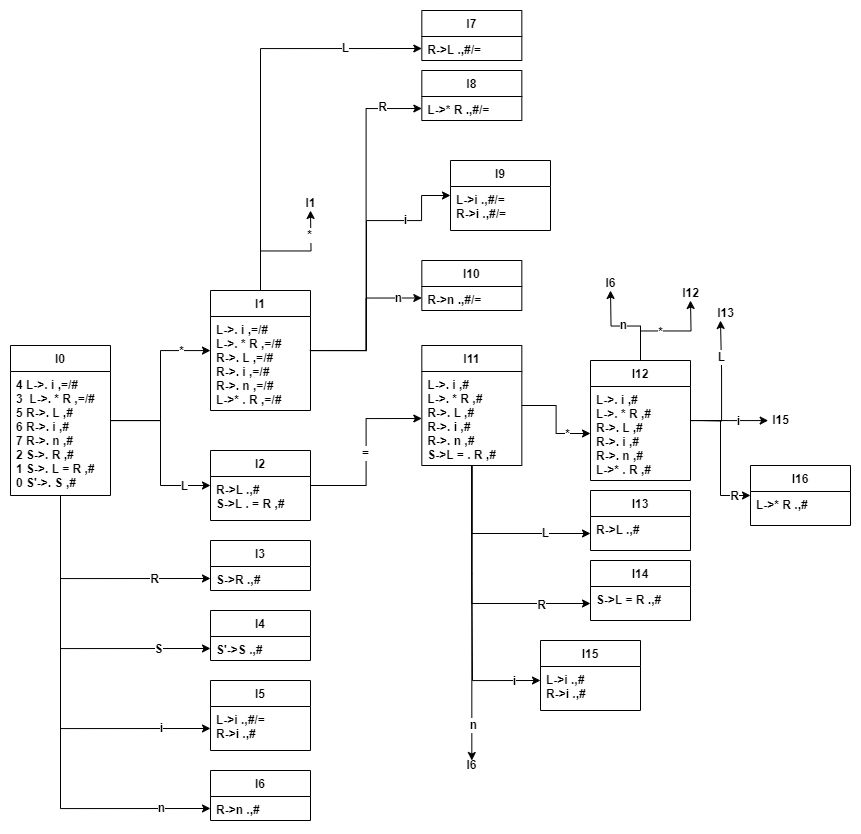
\includegraphics[width=0.8\textwidth]{photo/1.png}}
\vspace{10pt}

The table including the action table and goto table is provided:

\vspace{10pt}
\centerline{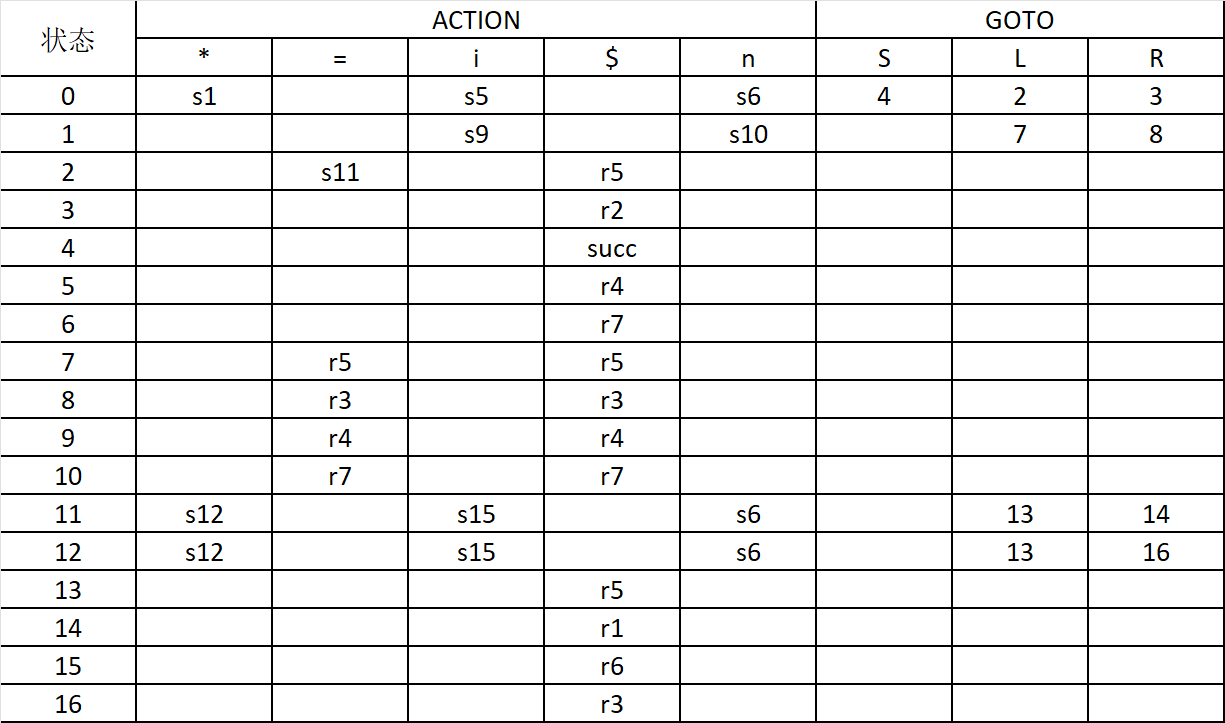
\includegraphics[width=0.8\textwidth]{photo/4.png}}
\vspace{10pt}

\section{Description of Important Data Structures}
\subsection{Class \texttt{LRAnalyseTable}}
This is the LR analysis table class.
\begin{lstlisting}[language=c++]
class LRParseTable {
    private:
        // Productions
        string grammar[15] = { "T->S", "S->L=R", "S->R", "L->*R", "L->i", "R->L", "R->i", "R->n" };
        // Terminals
        char terminalChars[10] = { '*', '=', 'i', '#', 'n' };
        // Non-terminals
        char nonTerminalChars[10] = { 'S', 'L', 'R' };
        // Number of terminals
        int numTerminals = 5;
        // Number of non-terminals
        int numNonTerminals = 3;
    
        // Action table
        int Action[20][5] = {
            {1, -1, 5, -1, 6}, {-1, -1, 9, -1, 10}, {-1, 11, -1, -15, -1}, {-1, -1, -1, -12, -1},
            {-1, -1, -1, 0, -1}, {-1, -1, -1, -14, -1}, {-1, -1, -1, -17, -1}, {-1, -15, -1, -15, -1},
            {-1, -13, -1, -13, -1}, {-1, -14, -1, -14, -1}, {-1, -17, -1, -17, -1}, {12, -1, 15, -1, 6},
            {12, -1, 15, -1, 6}, {-1, -1, -1, -15, -1}, {-1, -1, -1, -11, -1}, {-1, -1, -1, -16, -1}, {-1, -1, -1, -13, -1}
        };
        // Goto table
        int Goto[20][4] = {
            {4, 2, 3}, {-1, 7, 8}, {-1, -1, -1}, {-1, -1, -1}, {-1, -1, -1},
            {-1, -1, -1}, {-1, -1, -1}, {-1, -1, -1}, {-1, -1, -1},
            {-1, -1, -1}, {-1, -1, -1}, {-1, 13, 14}, {-1, 13, 16},
            {-1, -1, -1}, {-1, -1, -1}, {-1, -1, -1}, {-1, -1, -1}
        };
    
    public:
        LRParseTable() {}
        ~LRParseTable() {}
        int getTerminalIndex(char ch);
        int getNonTerminalIndex(char ch);
        int getAction(int state, char ch);
        int getGoto(int state, char ch);
        string getGrammar(int idx);
    };
\end{lstlisting}


\begin{itemize}
    \item \textbf{Member Variables}:
        - \texttt{grammar}: An array of strings storing all productions.
        - \texttt{terminalChars}: An array of characters storing terminals.
        - \texttt{nonTerminalChars}: An array of characters storing non-terminals.
        - \texttt{numTerminals}: The number of terminals.
        - \texttt{numNonTerminals}: The number of non-terminals.
        - \texttt{Action}: A 2D array representing the Action table.
        - \texttt{Goto}: A 2D array representing the Goto table.
    The Action table and Goto table are initialized as follows. -1 indicates no corresponding operation, i.e., the corresponding cell in the table is empty. Numbers less than -10 represent reductions. The production number used for reduction can be obtained by taking the opposite of the number plus 10 (the production number ranges from 0 to 7).
    \item \textbf{Member Functions}:
        - \texttt{getTerminalIndex(char ch)}: Gets the index of the terminal character in the terminal array.
        - \texttt{getNonTerminalIndex(char ch)}: Gets the index of the non-terminal character in the non-terminal array.
        - \texttt{getAction(int state, char ch)}: Queries the Action table based on the top state of the stack and the current symbol to get the corresponding action.
        - \texttt{getGoto(int state, char ch)}: Queries the Goto table based on the top state of the stack and the current symbol to get the corresponding action (used after reduction).
        - \texttt{getGrammar(int idx)}: Looks up the production array to get the corresponding production according to the production number used for reduction.
\end{itemize}

\subsection{Class \texttt{Analyser}}
This is the syntax analyzer class.
\begin{lstlisting}[language=c++]
class Parser {
    private:
        string inputString; // String to be parsed
        int step;           // Step count
        int currentIndex;   // Current index of the input string
        vector<char> symbolStack; // Symbol stack
        vector<int> stateStack;   // State stack
    public:
        Parser();
        ~Parser();
        bool startParsing(string input);
        string stackToString(int option);
    };
    Parser::Parser() {
        this->step = 1;
        this->currentIndex = 0;
        symbolStack.push_back('#');
        stateStack.push_back(0);
    }
\end{lstlisting}
\begin{itemize}
    \item \textbf{Member Variables}:
        - \texttt{inputString}: The string to be parsed.
        - \texttt{step}: The count of the current step.
        - \texttt{currentIndex}: The index of the current symbol in the input string.
        - \texttt{symbolStack}: A vector storing the symbol stack.
        - \texttt{stateStack}: A vector storing the state stack.
    \item \textbf{Member Functions}:
        - \texttt{Parser()}: Initializes the syntax analyzer. The step is initialized to 1, and the index of the current analyzed symbol is initialized to 0.
        - \texttt{stackToString(int option)}: Returns all the states or characters in the state stack or symbol stack for output display. This function selects whether to return the content in the state stack or the symbol stack according to the input parameter.
        - \texttt{startParsing(string input)}: The core analysis function. It determines whether the current character is legal. If it is legal, it performs a shift or reduce operation and modifies the symbol stack and state stack. After a reduction operation, the Goto table is queried to modify the state stack. The specific algorithm is described in the core algorithm section.
\end{itemize}

\section{Description of Core Algorithms}
The LR core algorithm is implemented in the \texttt{startParsing} function.
\begin{lstlisting}[language=c++]
bool Parser::startParsing(string input) {
    this->inputString = input;
    LRParseTable table;
    int currentState = 0;

    cout << setw(10) << "Step" << setw(15) << "State Stack" << setw(10)
            << "Symbol Stack" << setw(15) << "Current Symbol" << setw(15)
            << "Remaining String" << setw(20) << "Action" << endl;

    while (true) {
        int action = table.getAction(currentState, inputString[currentIndex]);
        if (action == 0) {
            cout << setw(10) << step << setw(15) << stackToString(0) << setw(10)
                    << stackToString(1) << setw(15) << inputString[currentIndex]
                    << setw(15) << inputString.substr(currentIndex) << setw(20)
                    << "Parsing complete" << endl;
            return true;
        }
        if (action == -1) {
            cerr << "Error: Unexpected symbol '" << inputString[currentIndex]
                    << "' at index " << currentIndex << endl;
            return false;
        }
        if (action > 0) {
            cout << setw(10) << step << setw(15) << stackToString(0) << setw(10)
                    << stackToString(1) << setw(15) << inputString[currentIndex]
                    << setw(15) << inputString.substr(currentIndex) << setw(20)
                    << "Action[S" << currentState << "][" << inputString[currentIndex]
                    << "]=S" << action << " (Shift)" << endl;
            stateStack.push_back(action);
            symbolStack.push_back(inputString[currentIndex]);
            currentIndex++;
        }
        else {
            int ruleIdx = -(action + 10);
            string rule = table.getGrammar(ruleIdx);
            if (rule.empty()) return false;

            cout << setw(10) << step << setw(15) << stackToString(0) << setw(10)
                    << stackToString(1) << setw(15) << inputString[currentIndex]
                    << setw(15) << inputString.substr(currentIndex) << setw(20)
                    << "R" << ruleIdx + 1 << ": " << rule << " (Reduce)" << endl;

            for (size_t i = 0; i < rule.size() - 3; i++) {
                if (stateStack.empty() || symbolStack.empty()) {
                    cerr << "Error: Stack underflow during reduction." << endl;
                    return false;
                }
                stateStack.pop_back();
                symbolStack.pop_back();
            }
            currentState = stateStack.back();
            int gotoResult = table.getGoto(currentState, rule[0]);
            if (gotoResult == -1) return false;
            cout << setw(10) << ++step << setw(15) << stackToString(0) << setw(10)
                    << stackToString(1) << setw(15) << rule[0] << setw(15)
                    << inputString.substr(currentIndex) << setw(20)
                    << "Goto[S" << currentState << "][" << rule[0] << "]=" << gotoResult
                    << " (State Transition)" << endl;
            stateStack.push_back(gotoResult);
            symbolStack.push_back(rule[0]);
        }
        currentState = stateStack.back();
        step++;
    }
}
    \end{lstlisting}
First, initialization is performed. The input string is stored in \texttt{inputString}, the step number \texttt{step} is set to 1, the current index \texttt{currentIndex} is set to 0, `\#' is pushed onto the symbol stack \texttt{symbolStack}, and the initial state 0 is pushed onto the state stack \texttt{stateStack}. Then, it enters the loop analysis stage. The action \texttt{action} corresponding to the current state \texttt{currentState} and the current position \texttt{inputString[currentIndex]} of the input string is obtained, and different types of action judgments are made according to the value of \texttt{action}: If \texttt{action == 0}, it indicates that the analysis is successful, the analysis completion information is output, and \texttt{true} is returned; if \texttt{action == -1}, it means that an unexpected symbol is encountered, an error message is output, and \texttt{false} is returned; if \texttt{action > 0}, a shift operation is performed, that is, the state \texttt{action} is pushed onto the state stack, the current symbol \texttt{inputString[currentIndex]} is pushed onto the symbol stack, and then \texttt{currentIndex} is incremented by 1; if \texttt{action < 0}, a reduce operation is performed. First, the index \texttt{ruleIdx} of the grammar production to be applied is calculated according to \texttt{action}. Then, the same number of elements as the number of symbols on the right side of the production are popped from the symbol stack and the state stack. After that, the current state \texttt{currentState} is obtained, and the transition state \texttt{gotoResult} after applying the production is calculated. Finally, \texttt{gotoResult} is pushed onto the state stack, and the left side symbol of the production is pushed onto the symbol stack. After completing an action judgment, the current state is updated to the top element of the state stack, and the step number \texttt{step} is incremented. This loop continues until the analysis is completed.

The \texttt{main} function is as follows:
\begin{lstlisting}[language=c++]
int main() {
    FILE* in;
    FILE* out;
    if (freopen_s(&in, "test.txt", "r", stdin)!= 0) {
        cerr << "Error: Unable to open test.txt for reading." << endl;
        return 1;
    }
    if (freopen_s(&out, "result.txt", "w", stdout)!= 0) {
        cerr << "Error: Unable to open result.txt for writing." << endl;
        return 1;
    }

    string str;
    int caseCount = 1;
    while (getline(cin, str)) {
        cout << "Case " << caseCount++ << ": " << str << endl;
        Parser parser;
        if (parser.startParsing(str)) {
            cout << "The input string '" << str << "' is valid." << endl;
        }
        else {
            cout << "The input string '" << str << "' is invalid." << endl;
        }
        cout << endl;
    }
    return 0;
}
\end{lstlisting}
In the \texttt{main} function, the program reads the input string from the \texttt{test.txt} file, performs LR analysis on each input string, and outputs the result to the \texttt{result.txt} file.

\section{Use Cases on Running}
The test cases are in the \texttt{test.txt} file:
\begin{lstlisting}
i=i#
*i=i#
*i#
i#
=i#
ii#
\end{lstlisting}
The terminal output results are as follows:
\begin{lstlisting}
Error: Unexpected symbol '=' at index 1
Error: Unexpected symbol '=' at index 0
Error: Unexpected symbol 'i' at index 1
\end{lstlisting}
The output results in the \texttt{result.txt} file:

\vspace{10pt}
\centerline{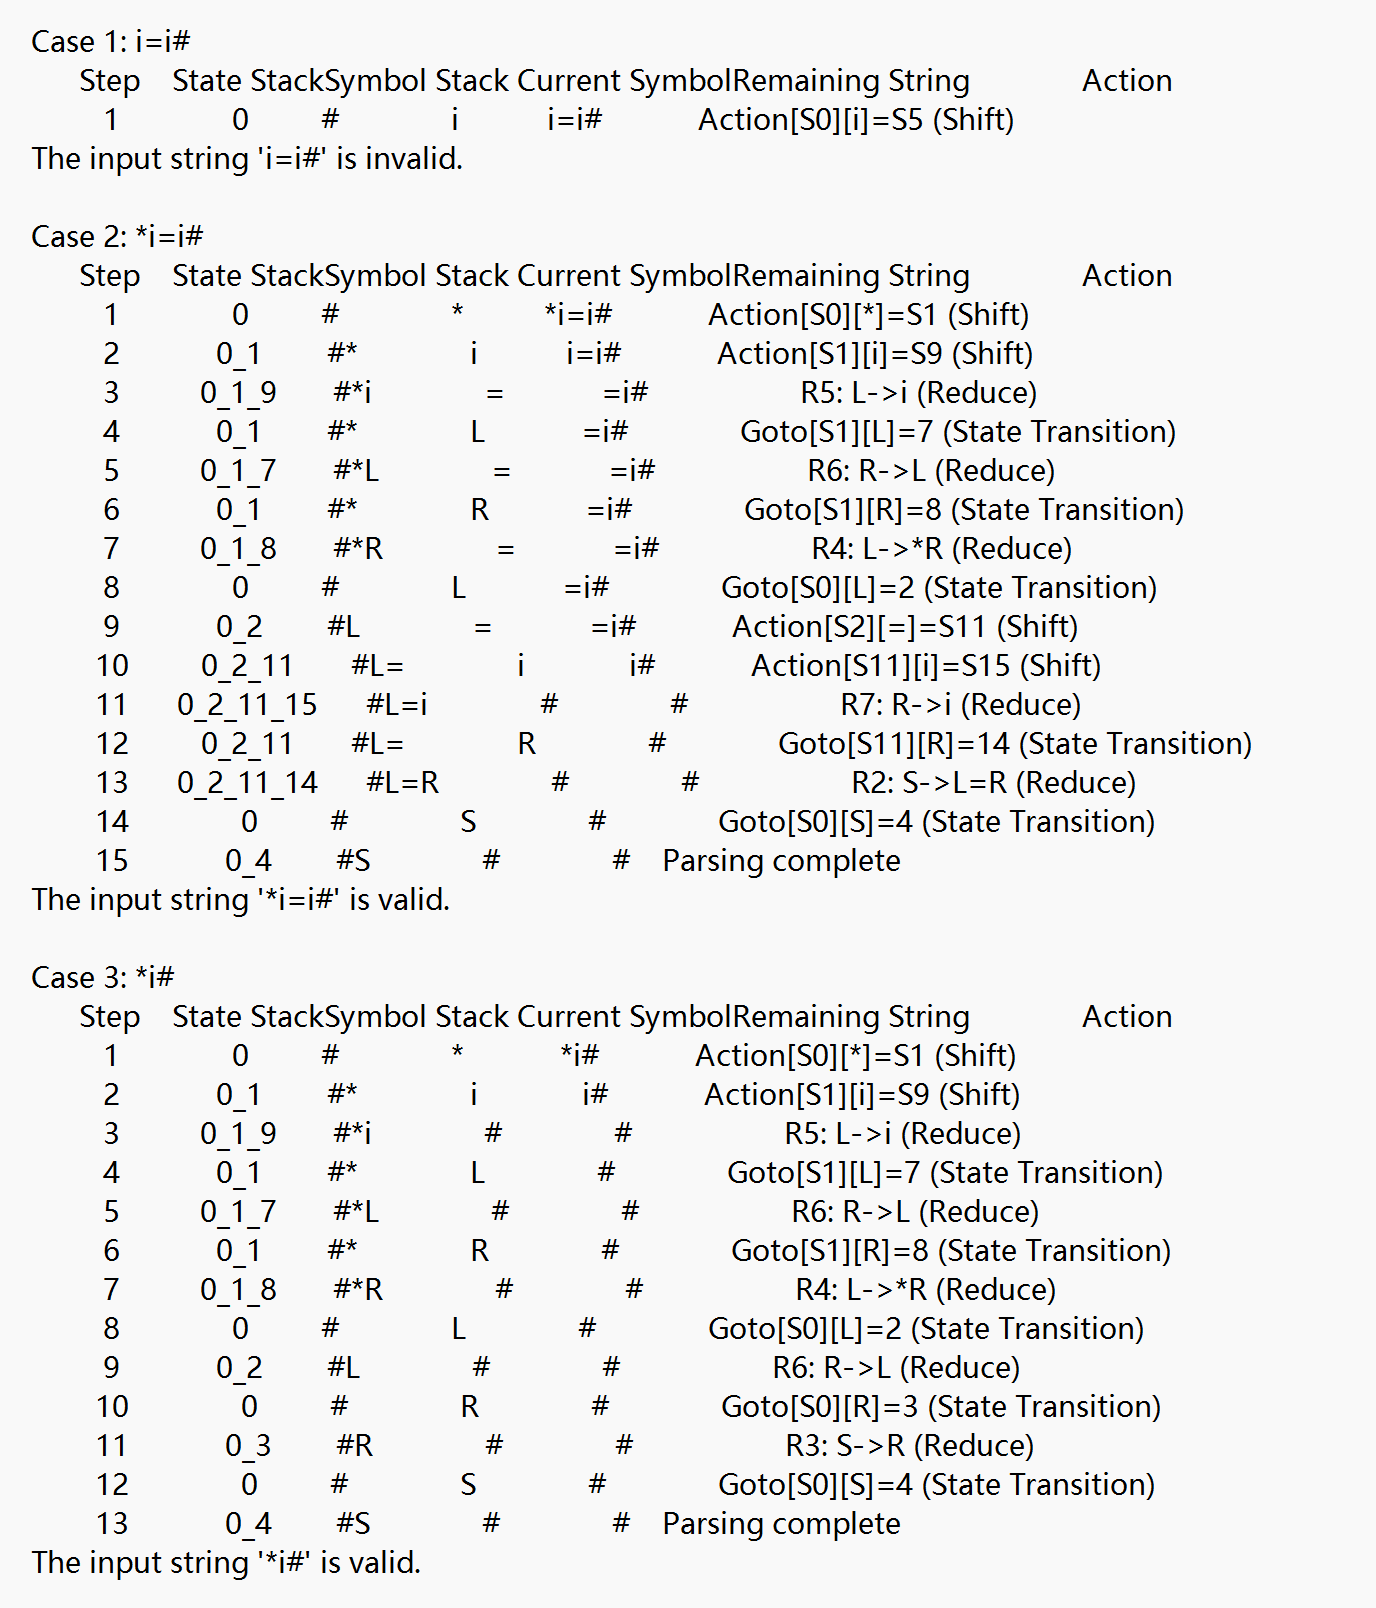
\includegraphics[width=0.8\textwidth]{photo/2.png}}
\vspace{10pt}

\centerline{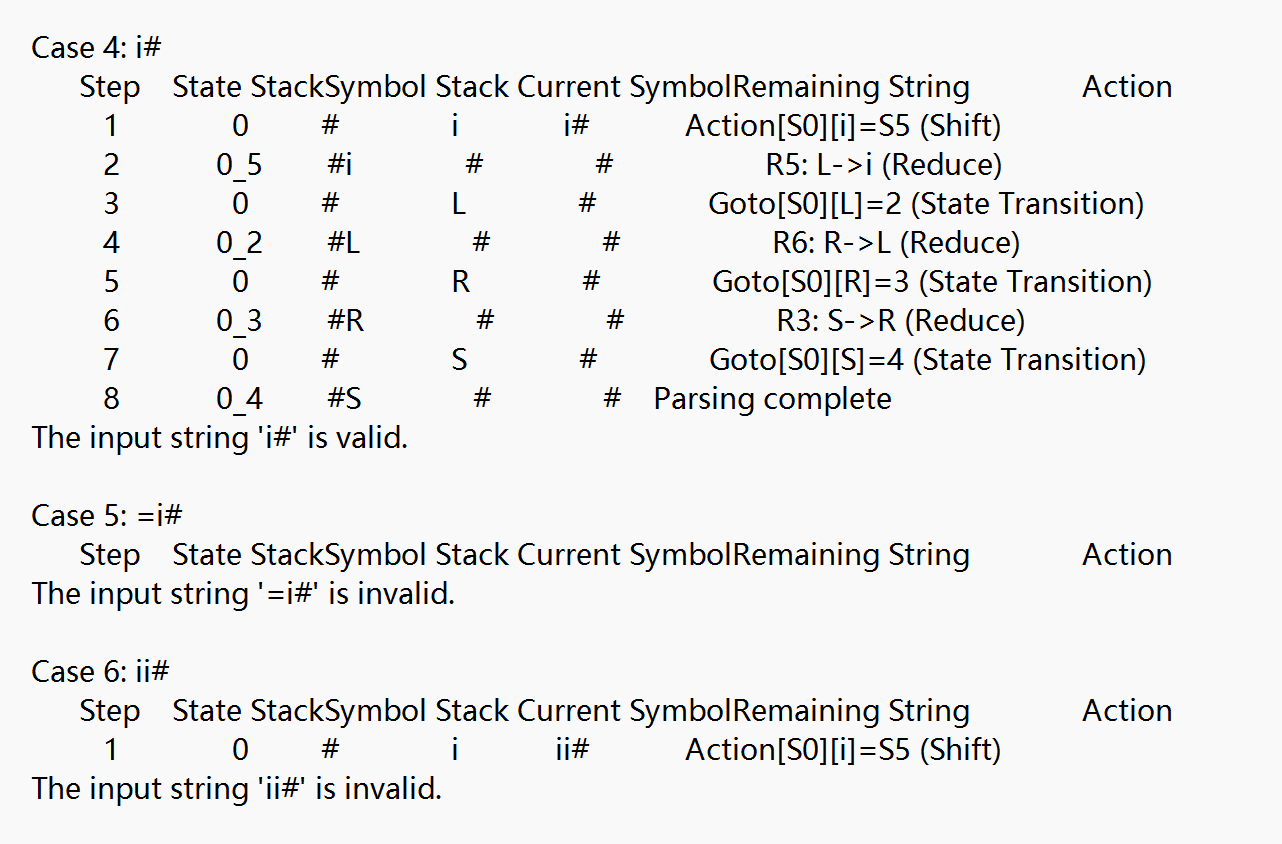
\includegraphics[width=0.8\textwidth]{photo/3.png}}
\vspace{10pt}

\section{Problems Occurred and Related Solutions}
Initially, there were errors in the construction of the action table and Goto table, resulting in incorrect program running results and the parser entering an infinite loop. Later, this problem was manually solved, and the program was able to run accurately.

In the ACTION table, there are both shift and reduce operations. To distinguish these two operations, reduce operations are represented by negative numbers less than -10. The specific conversion method is: take the opposite of the production number used for reduction plus 10.

The number of elements popped from the state stack and the symbol stack was incorrect, resulting in an attempt to access an empty stack. I modified the code responsible for the reduce operation so that it can correctly calculate the number of symbols to be popped according to the length of the production rule.

\section{Feelings and Comments}
\begin{enumerate}
    \item Through this experiment, I have a deeper understanding of LR(1) analysis. Since it is a bottom-up analysis method, the characters to be analyzed can be scanned and analyzed at the same time. Before constructing an LR(1) syntax analyzer, some preparatory operations are required. First, a DFA needs to be drawn. For LR(1) analysis, one more symbol needs to be looked ahead. Therefore, LR(1) items not only include productions but also need to carry lookahead symbols. Even if the productions are the same, different lookahead symbols represent different states. Then, the ACTION and GOTO tables need to be drawn based on the DFA and used to write the program.
    \item After reduction, the GOTO table needs to be queried to update the top of the state stack according to the updated symbol stack and the symbol and state at the top of the state stack. This is a detail that I did not notice in previous studies. At the same time, it also reflects the role of the GOTO table. Before the experiment, I was not very clear why there are two tables, ACTION and GOTO. After this experiment, I understand it more deeply.
\end{enumerate}

\end{document}